\chapter{Resultados} \label{cap:results}
Neste capítulo são apresentados os resultados obtidos do trabalho desenvolvido. Primeiramente, os resultados de negócio envolvidos na implementação da aplicação são apresentados. Em seguida, uma comparação das ferramentas de teste automatizado é feita. Por último, são discutidos os resultados obtidos do ponto de vista da empresa em que este projeto esteve inserido.

\section{Versão Piloto}
\subsection{Uso do Aplicativo}
O desenvolvimento do aplicativo para o sistema iOS, apresentado neste trabalho, culminou no lançamento da sua versão piloto. Esta versão consiste na primeira etapa de lançamentos do produto e tem como objetivo a validação da ideia. O aplicativo piloto foi avaliado por um grupo seleto de academias e treinadores, localizados em Sydney.

A Figura \ref{fig:pilot-use} ilustra a utilização da versão piloto do aplicativo, com dados coletados da ferramenta Fabric. O gráfico mostra o número de usuários ativos diariamente desde o lançamento do piloto. O eixo horizontal representa a evolução temporal em dias, enquanto o eixo vertical contém o número total de usuários diários. O primeiro pico (entre os dias 10 e 28 de outubro) corresponde a distribuição de um incremento da versão piloto, ultrapassando o número de 10 usuários. O segundo e o terceiro picos (entre os dias 4 e 11 de novembro) dizem respeito a uma nova versão de incremento do piloto, com o convite de mais parceiros para o teste do aplicativo. Totalizando 19 usuários utilizando a aplicação.

\begin{figure}[H]
    \centering
    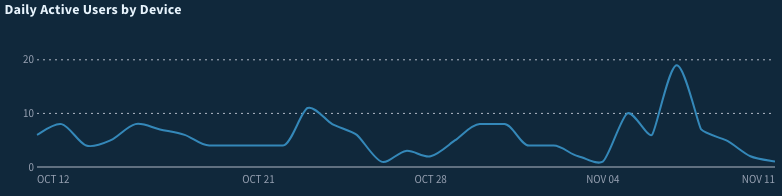
\includegraphics[width=\textwidth]{pfc/figuras/pilot-use.png}
    \caption{Uso diário da versão piloto do aplicativo}
    \label{fig:pilot-use}
\end{figure}

\subsection{Desenvolvimento do Produto}
O resultado da implementação da aplicação, no período contemplado neste PFC de aproximadamente 4 meses, contribuíram para grandes avanços no desenvolvimento do produto. A versão atual do aplicativo para o sistema iOS totaliza 33 telas principais de interação com o usuário (Figura \ref{fig:all-screens}). Estas interfaces permitem que os seguintes fluxos de atividade sejam realizados pelos usuários finais do produto:
\begin{itemize}
    \item Cadastro de academias;
    \item Cadastro de treinadores;
    \item Construção de agenda semanal de blocos para locação nas academias;
    \item Acompanhamento diário de sessões de treino agendadas nas academias;
    \item Visualização de dados semanais das academias em dashboard;
    \item Visualização e edição de perfil das academias;
    \item Busca por academias disponíveis em mapa dinâmico;
    \item Adição de academias à seleção de favoritos;
    \item Visualização de agenda diária dos treinadores;
    \item Cancelamento e avaliação de sessões de treino;
    \item Visualização e edição de perfil de treinador;
    \item Visualização de dados semanais dos treinadores em dashboard;
    \item Visualização de disponibilidade diária de blocos de academias através de calendário;
    \item Agendamento de sessão de treino.
\end{itemize}
\begin{figure}[H]
	\centering
    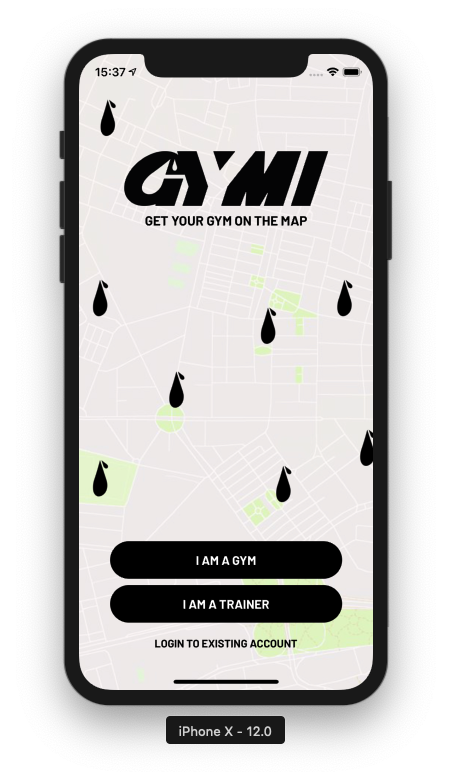
\includegraphics[width=0.14\textwidth]{pfc/figuras/landing.png}
    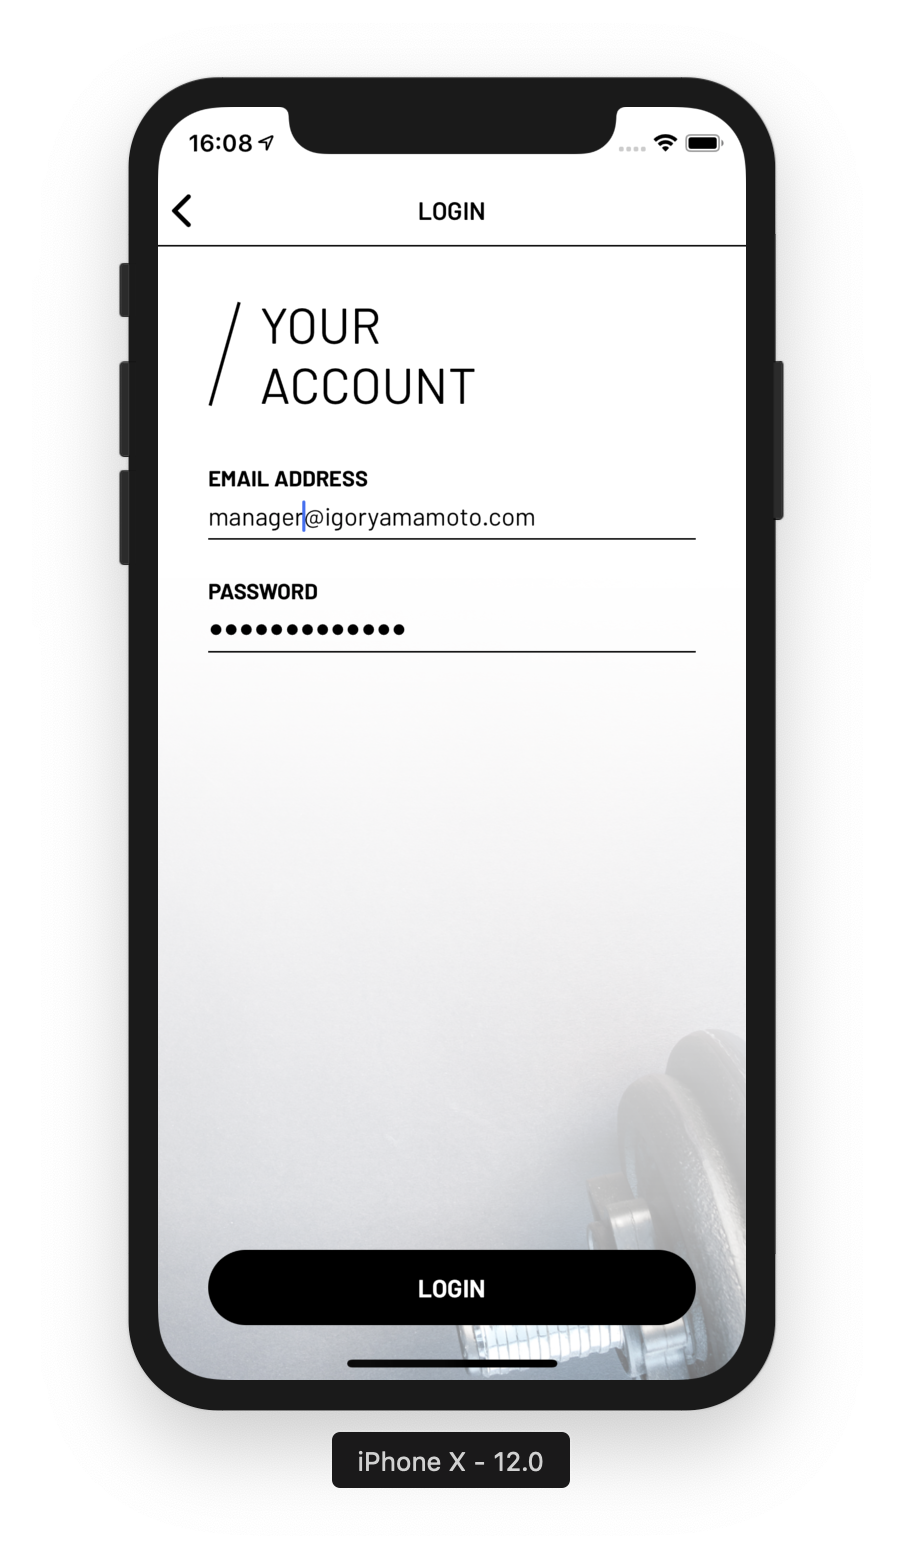
\includegraphics[width=0.14\textwidth]{pfc/figuras/login.png}
    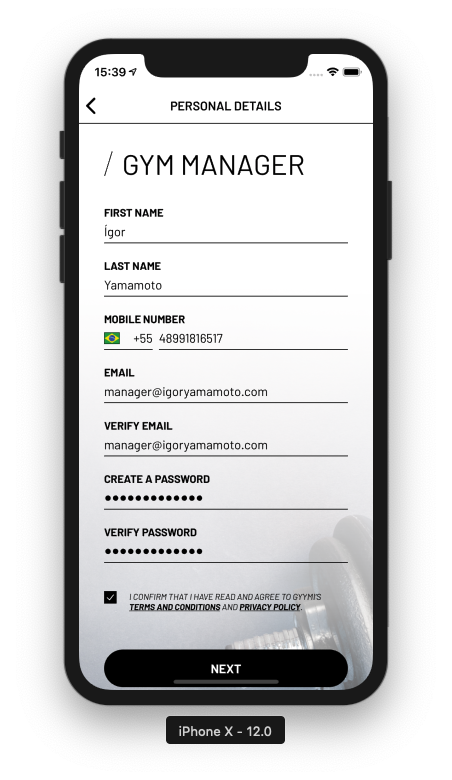
\includegraphics[width=0.14\textwidth]{pfc/figuras/register-manager.png}
    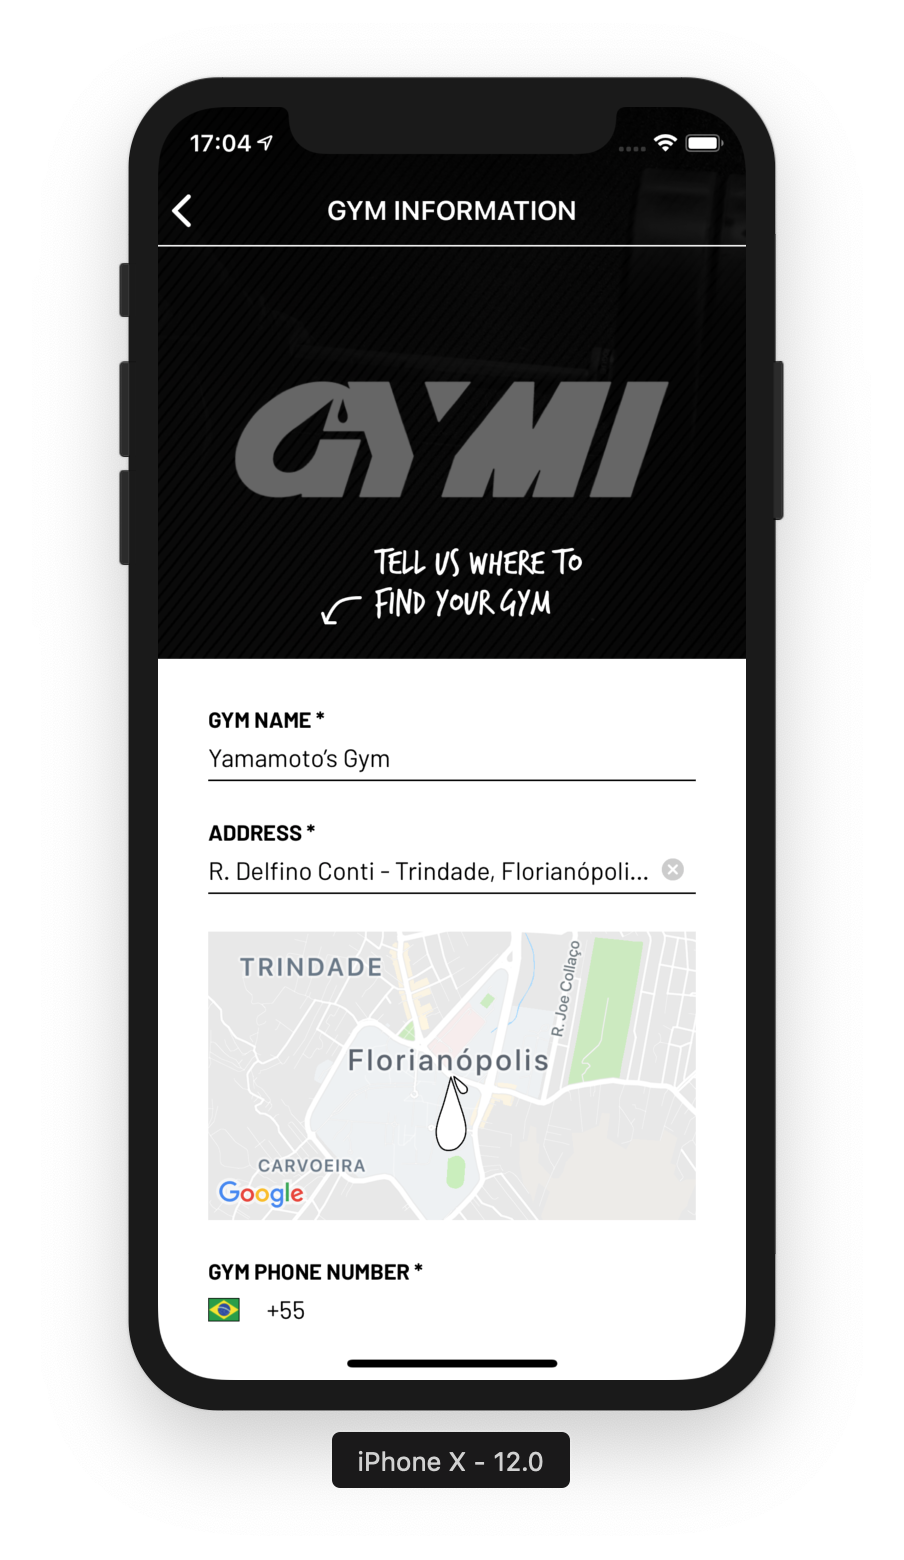
\includegraphics[width=0.14\textwidth]{pfc/figuras/register-gym-info.png}
    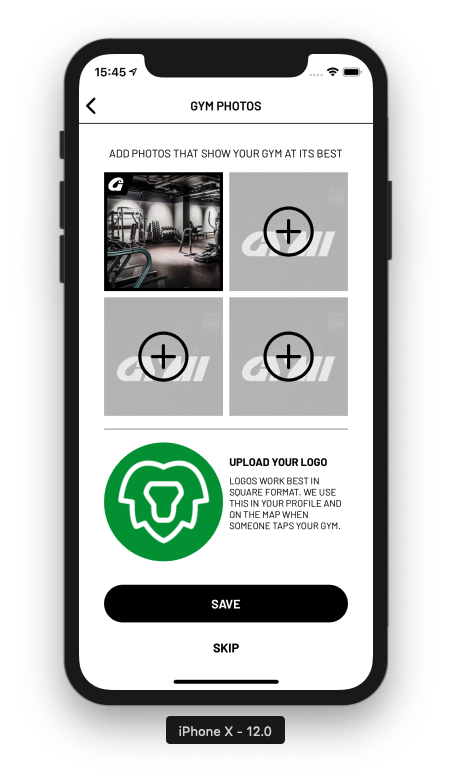
\includegraphics[width=0.14\textwidth]{pfc/figuras/register-gym-photos.png}
    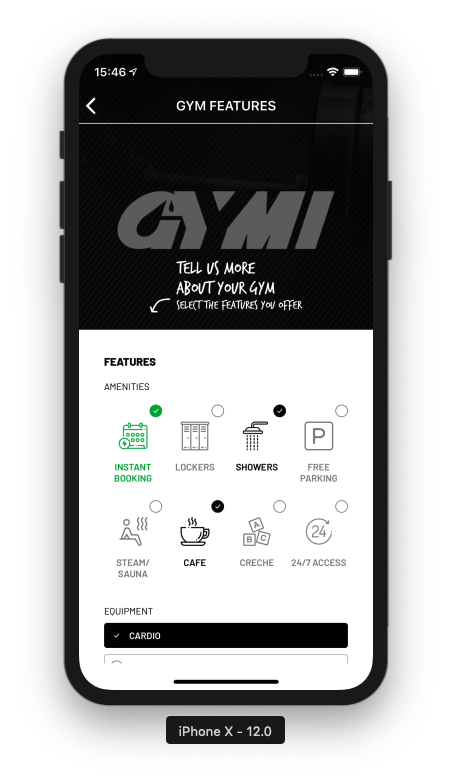
\includegraphics[width=0.14\textwidth]{pfc/figuras/register-gym-amenities.png}
    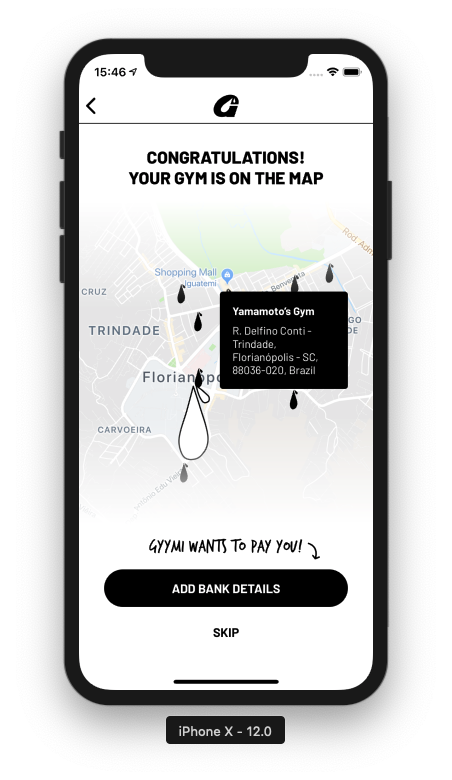
\includegraphics[width=0.14\textwidth]{pfc/figuras/gym-welcome.png}
    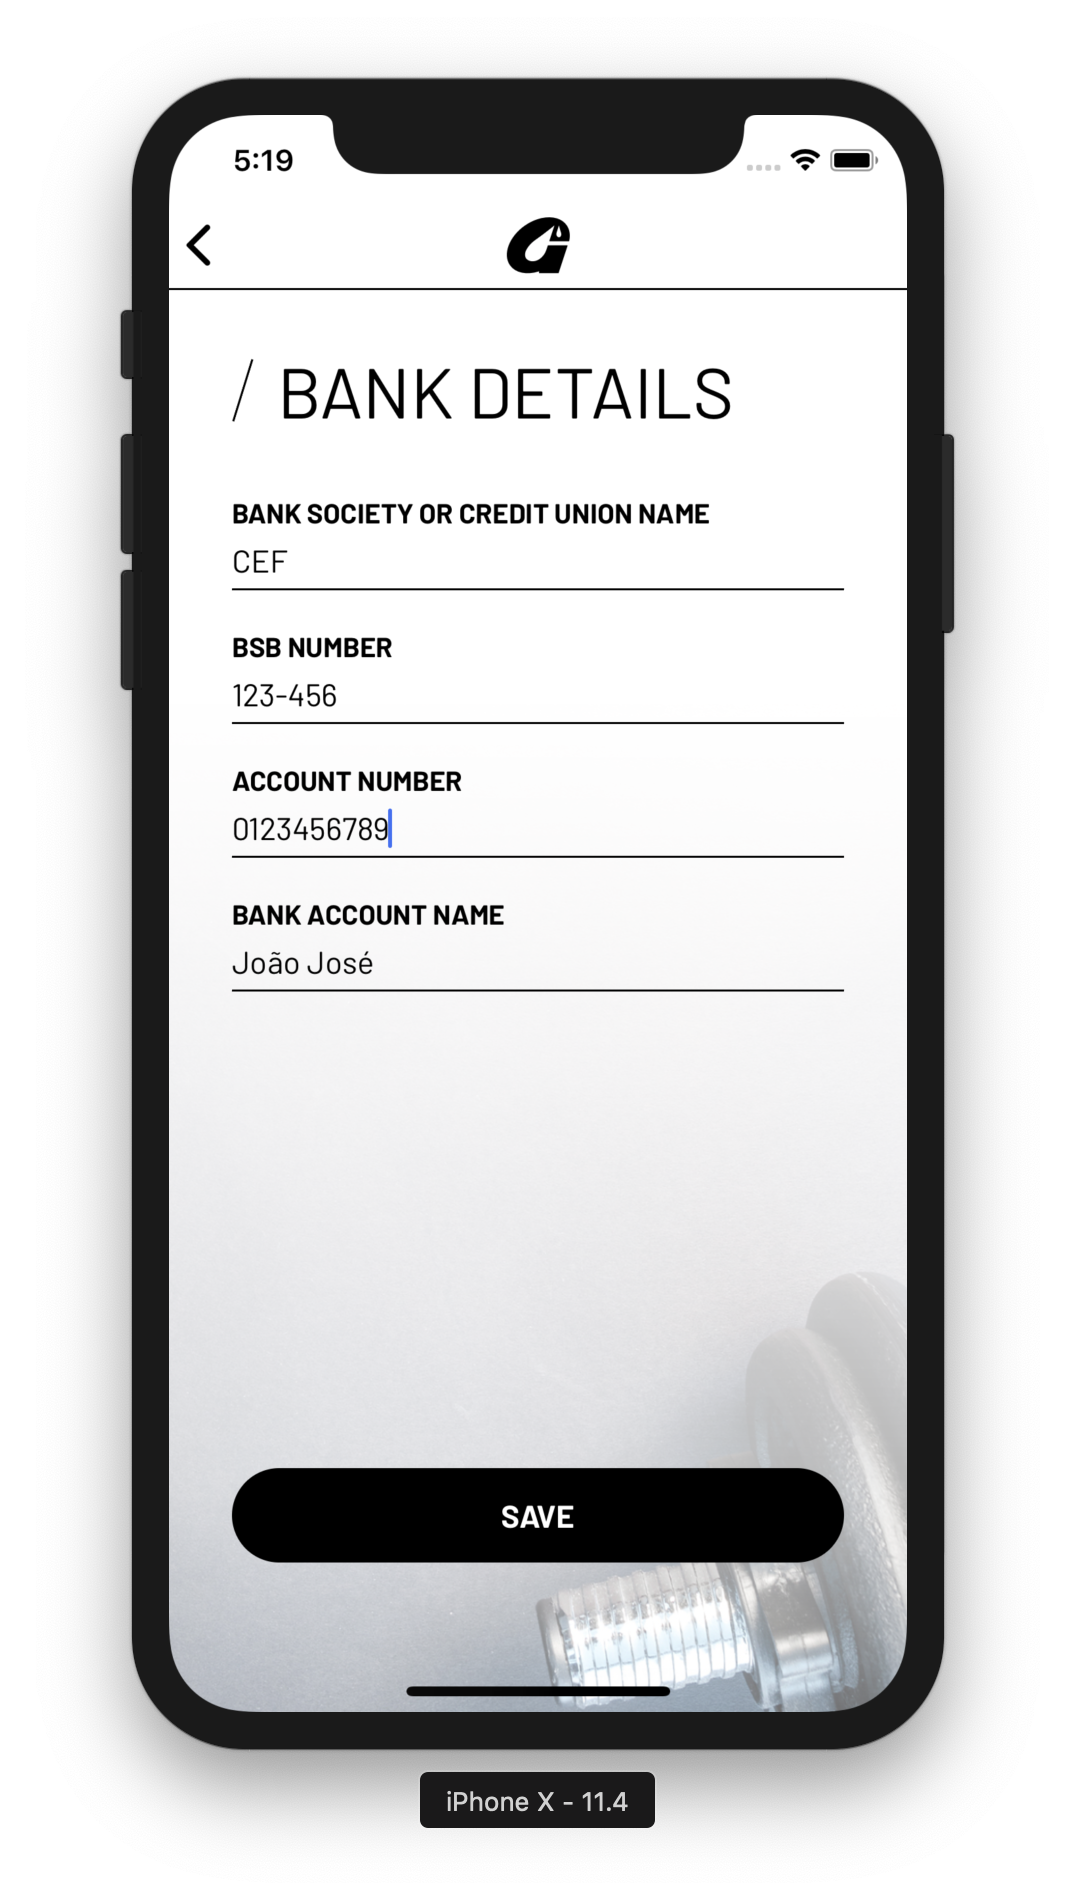
\includegraphics[width=0.14\textwidth]{pfc/figuras/bank-details.png}
    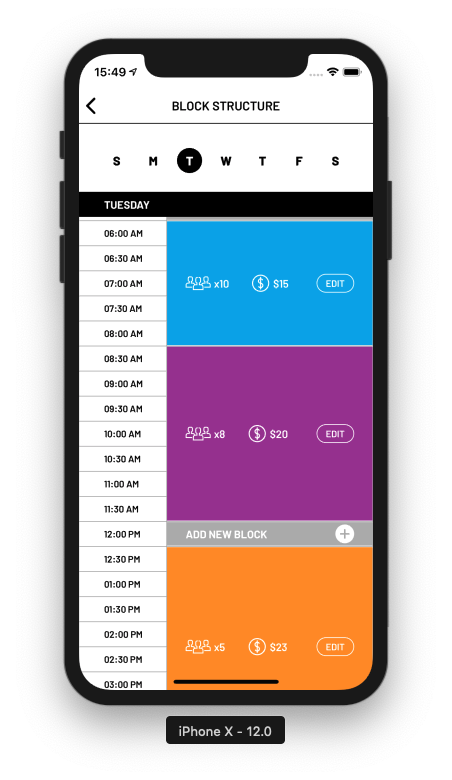
\includegraphics[width=0.14\textwidth]{pfc/figuras/gym-block-structure.png}
    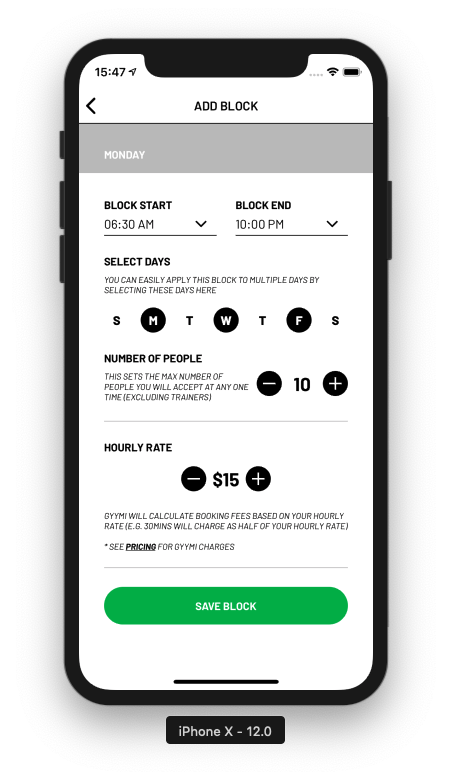
\includegraphics[width=0.14\textwidth]{pfc/figuras/gym-add-block.png}
    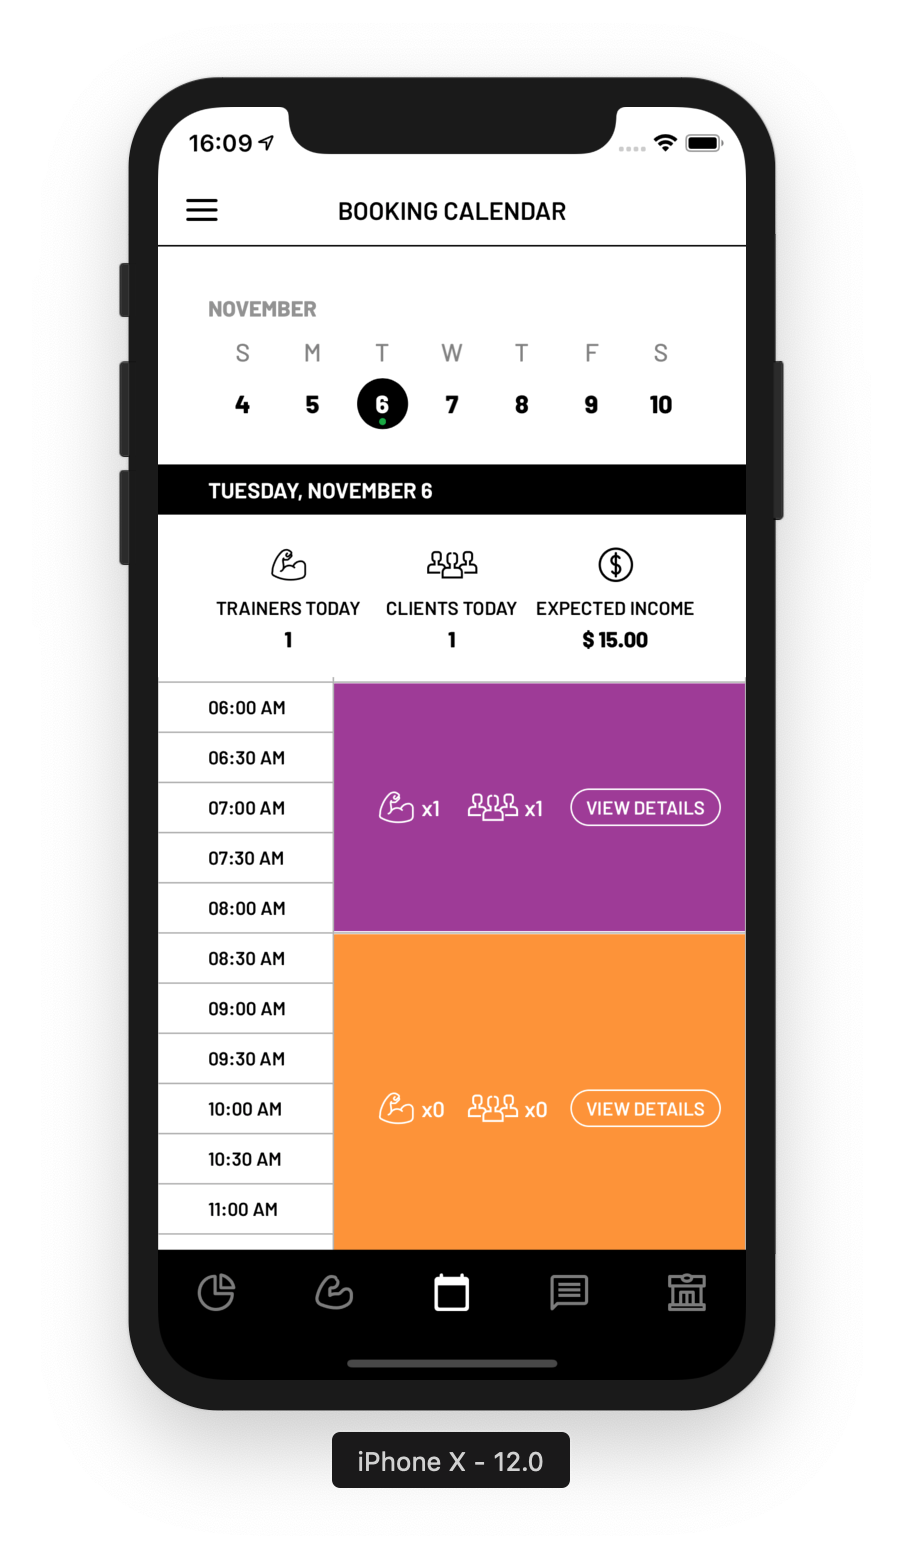
\includegraphics[width=0.14\textwidth]{pfc/figuras/gym-booking-calendar.png}
    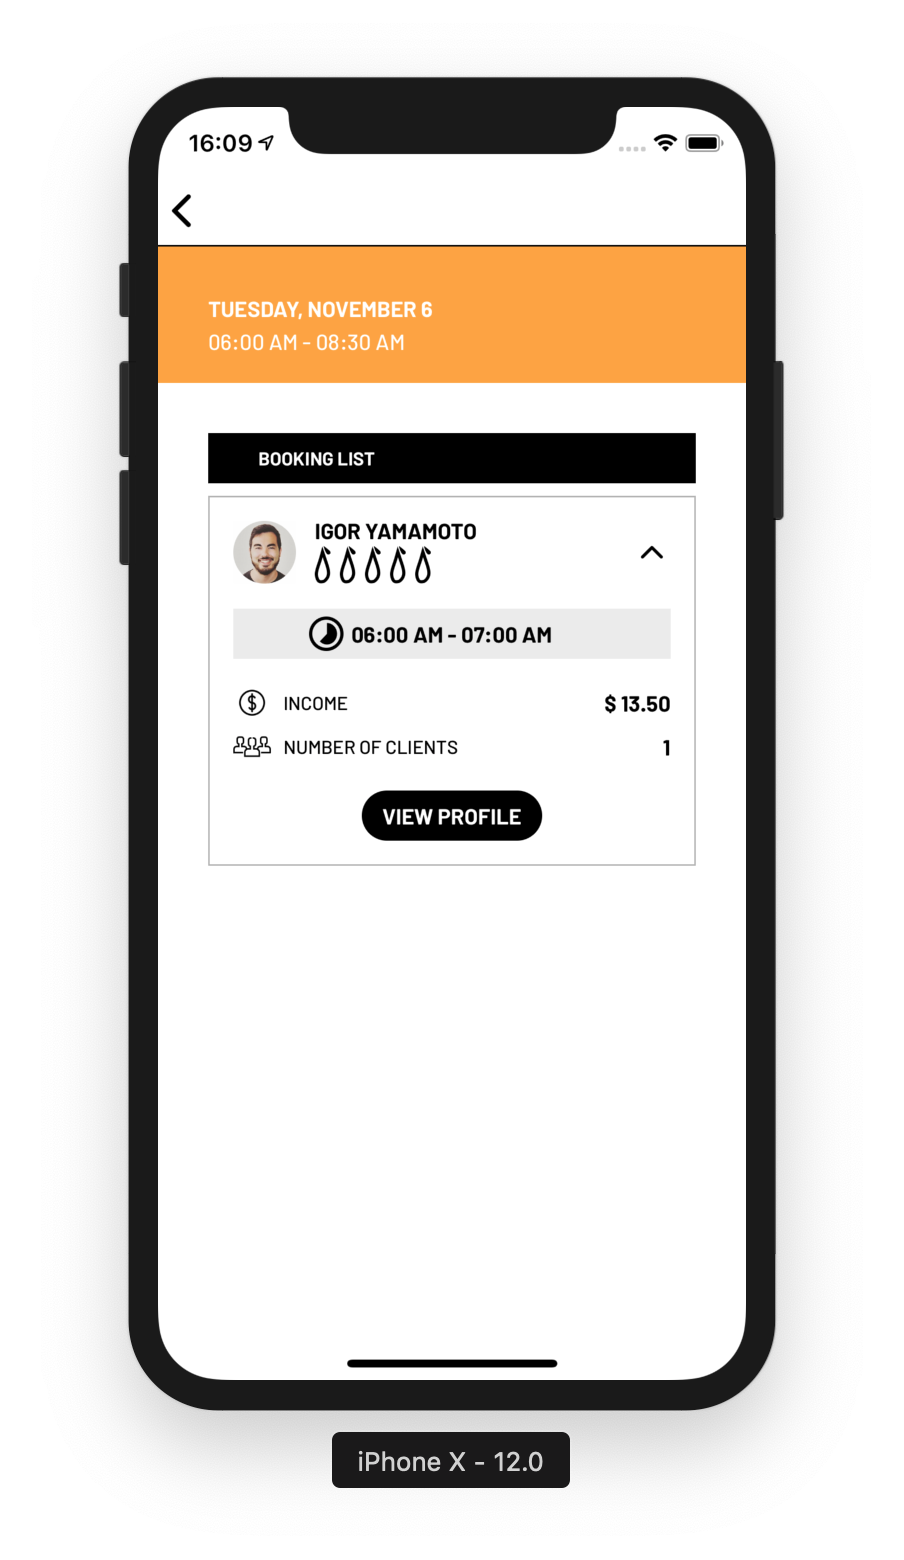
\includegraphics[width=0.14\textwidth]{pfc/figuras/gym-booking-detail.png}
    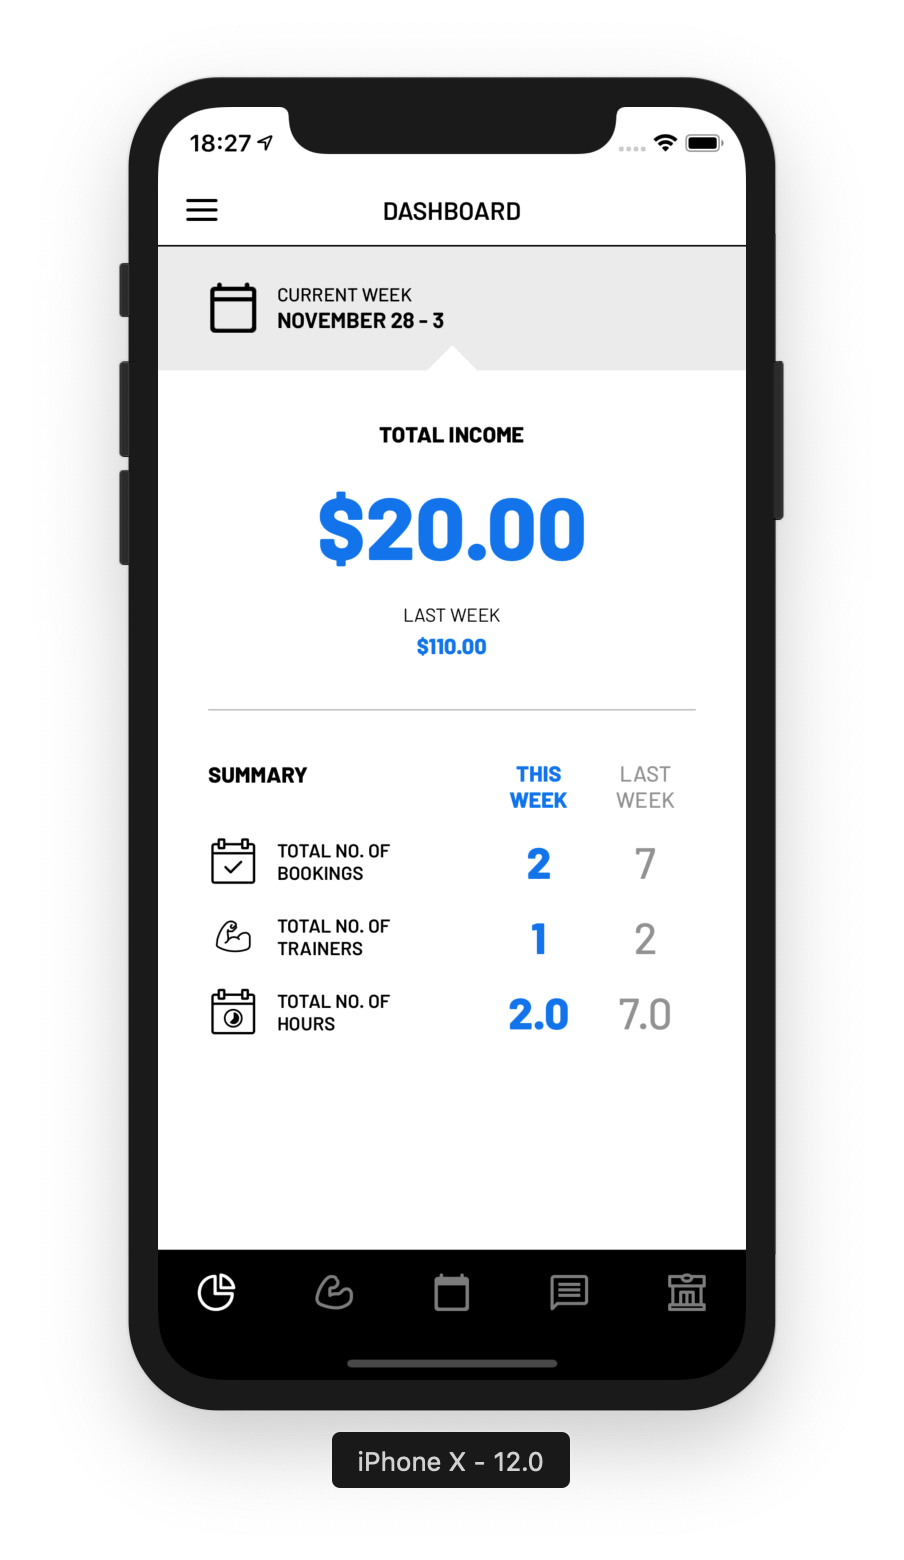
\includegraphics[width=0.14\textwidth]{pfc/figuras/gym-dashboard.png}
    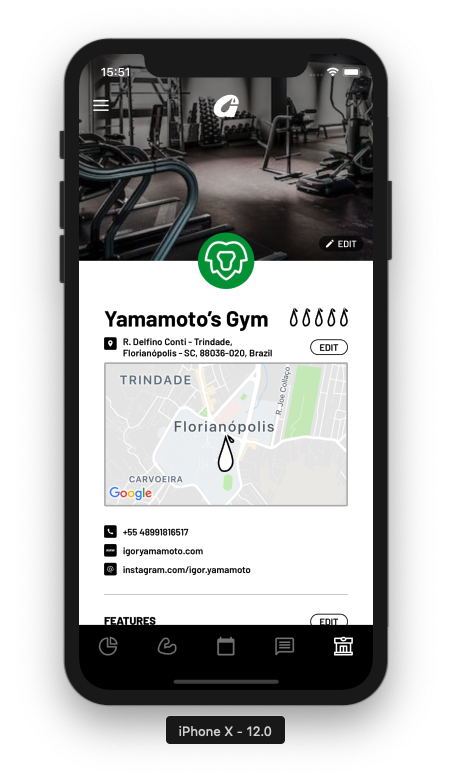
\includegraphics[width=0.14\textwidth]{pfc/figuras/gym-profile.png}
    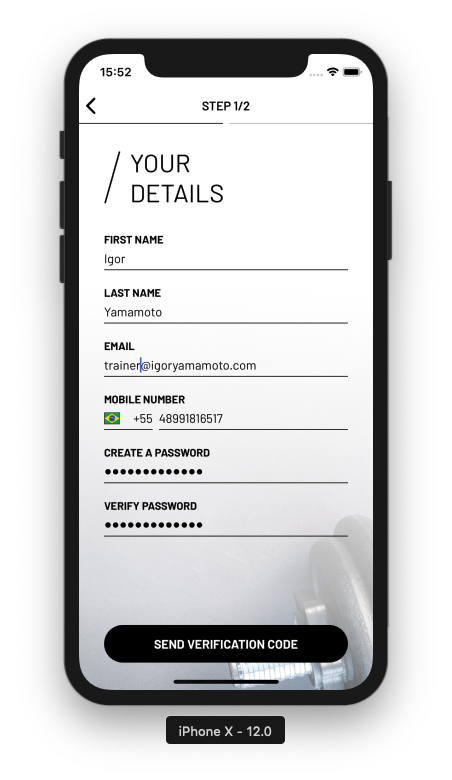
\includegraphics[width=0.14\textwidth]{pfc/figuras/register-trainer.png}
    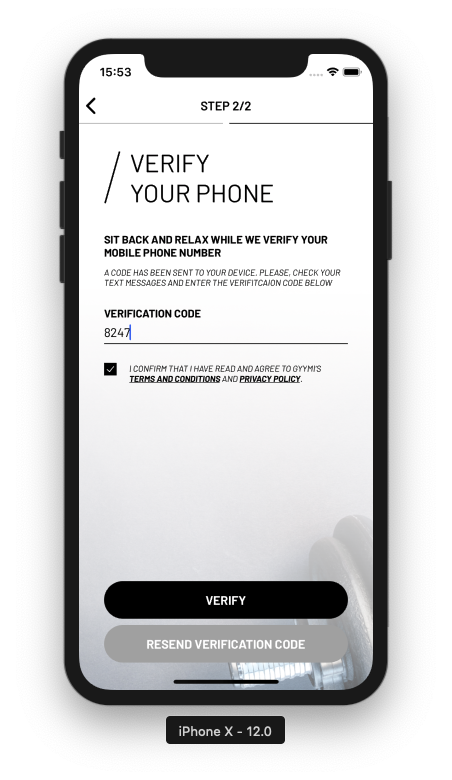
\includegraphics[width=0.14\textwidth]{pfc/figuras/register-trainer-verification.png}
    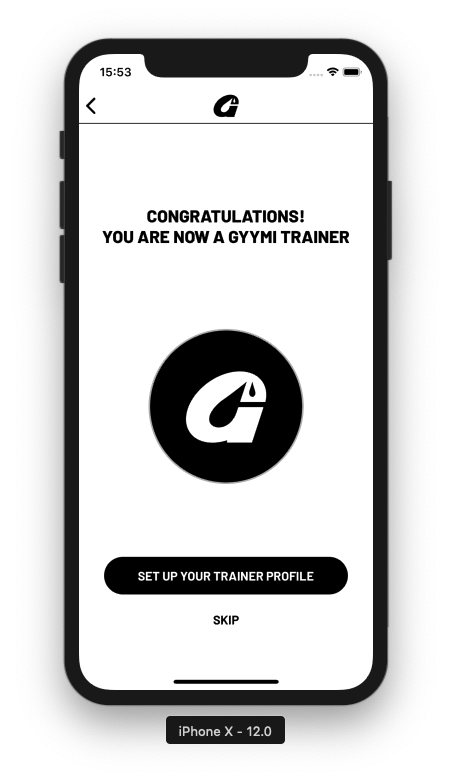
\includegraphics[width=0.14\textwidth]{pfc/figuras/tr-congratulations.png}
    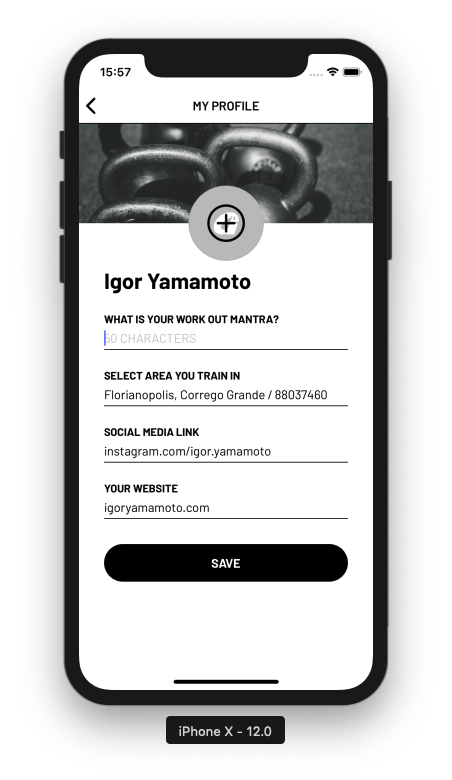
\includegraphics[width=0.14\textwidth]{pfc/figuras/tr-register-profile-1.png}
    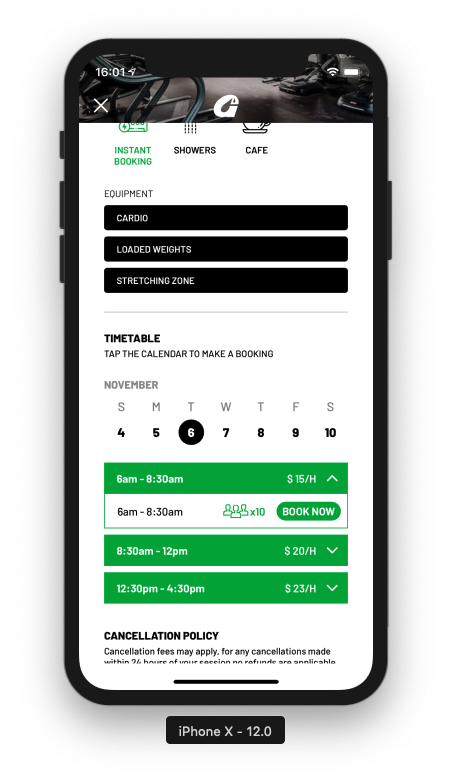
\includegraphics[width=0.14\textwidth]{pfc/figuras/tr-gym-profile-2.png}
    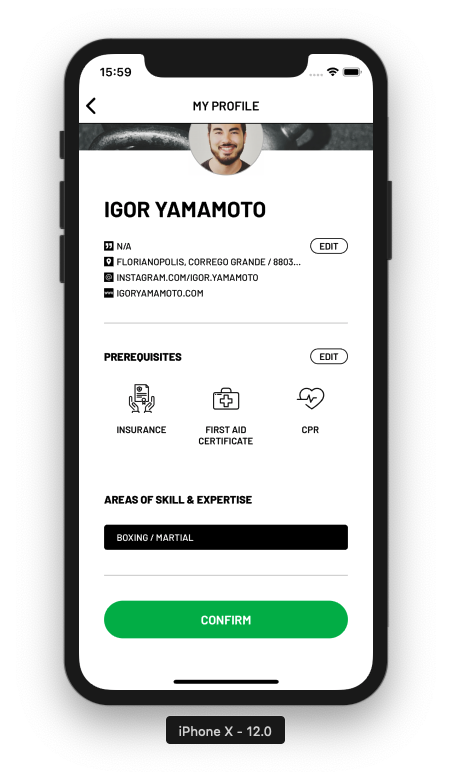
\includegraphics[width=0.14\textwidth]{pfc/figuras/tr-register-profile-3.png}
    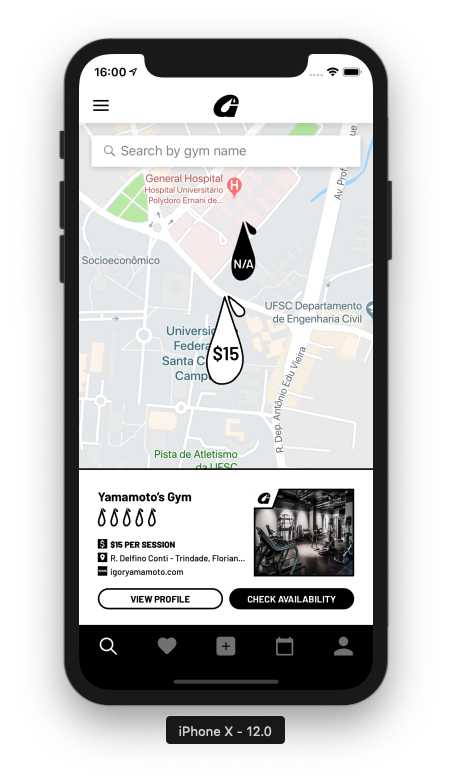
\includegraphics[width=0.14\textwidth]{pfc/figuras/tr-home-map.png}
    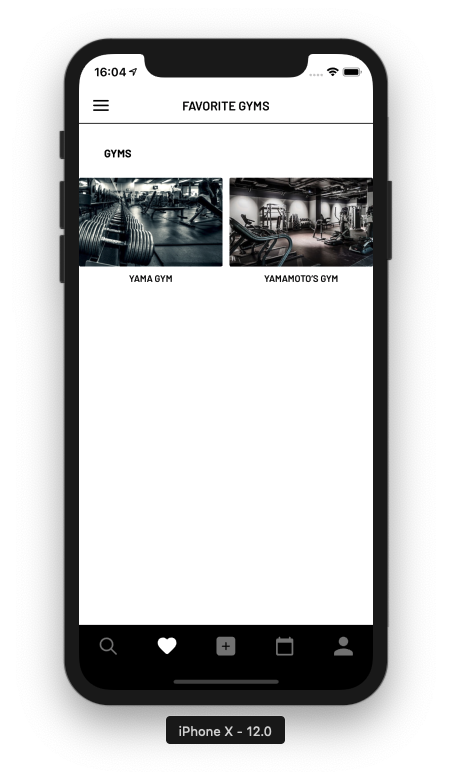
\includegraphics[width=0.14\textwidth]{pfc/figuras/tr-favorite.png}
    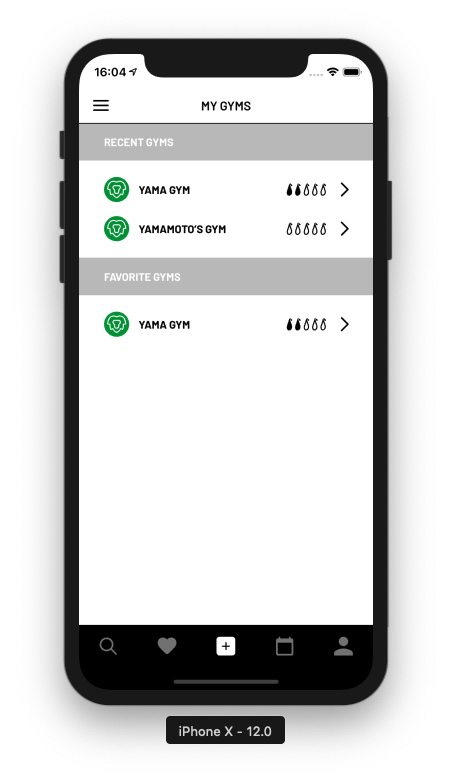
\includegraphics[width=0.14\textwidth]{pfc/figuras/tr-my-gyms.png}
    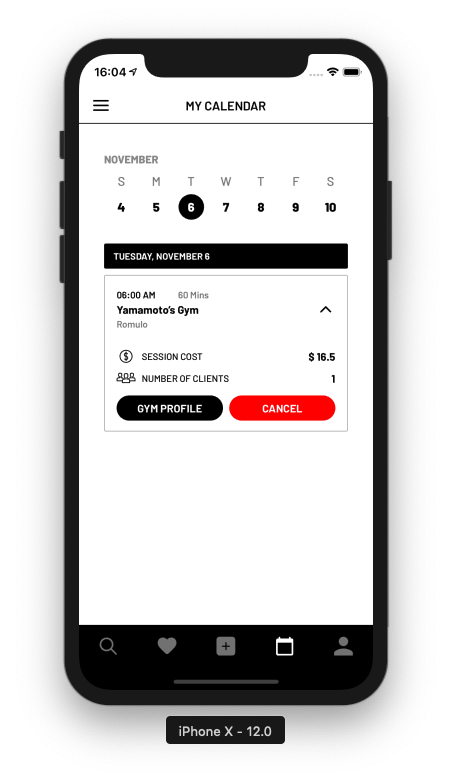
\includegraphics[width=0.14\textwidth]{pfc/figuras/tr-calendar.png}
    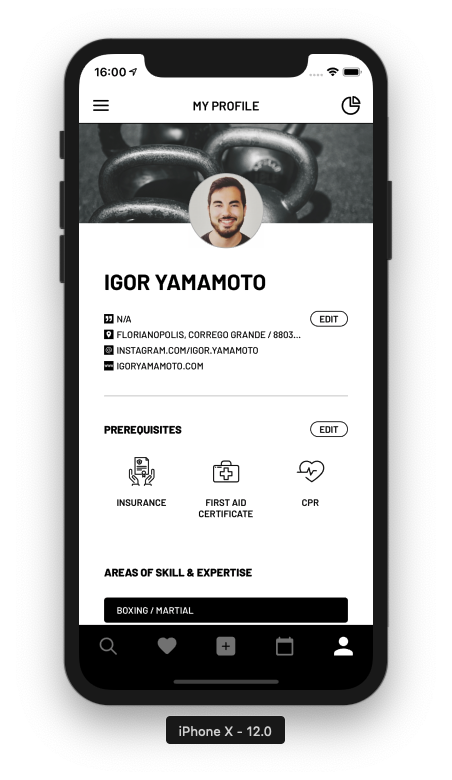
\includegraphics[width=0.14\textwidth]{pfc/figuras/tr-profile.png}
    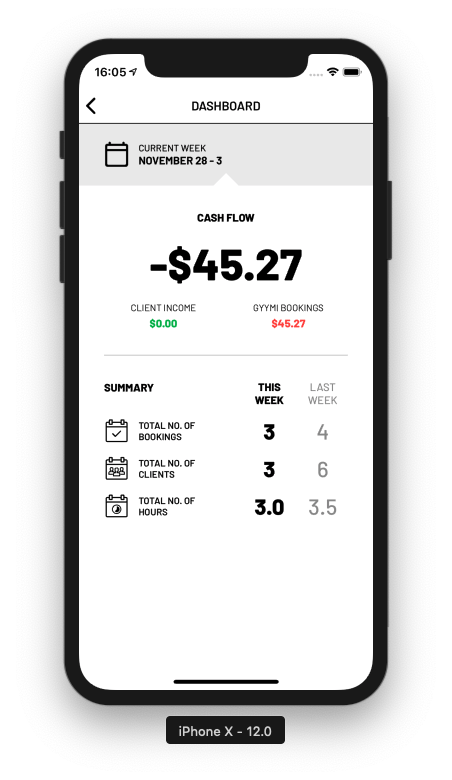
\includegraphics[width=0.14\textwidth]{pfc/figuras/tr-dashboard.png}
    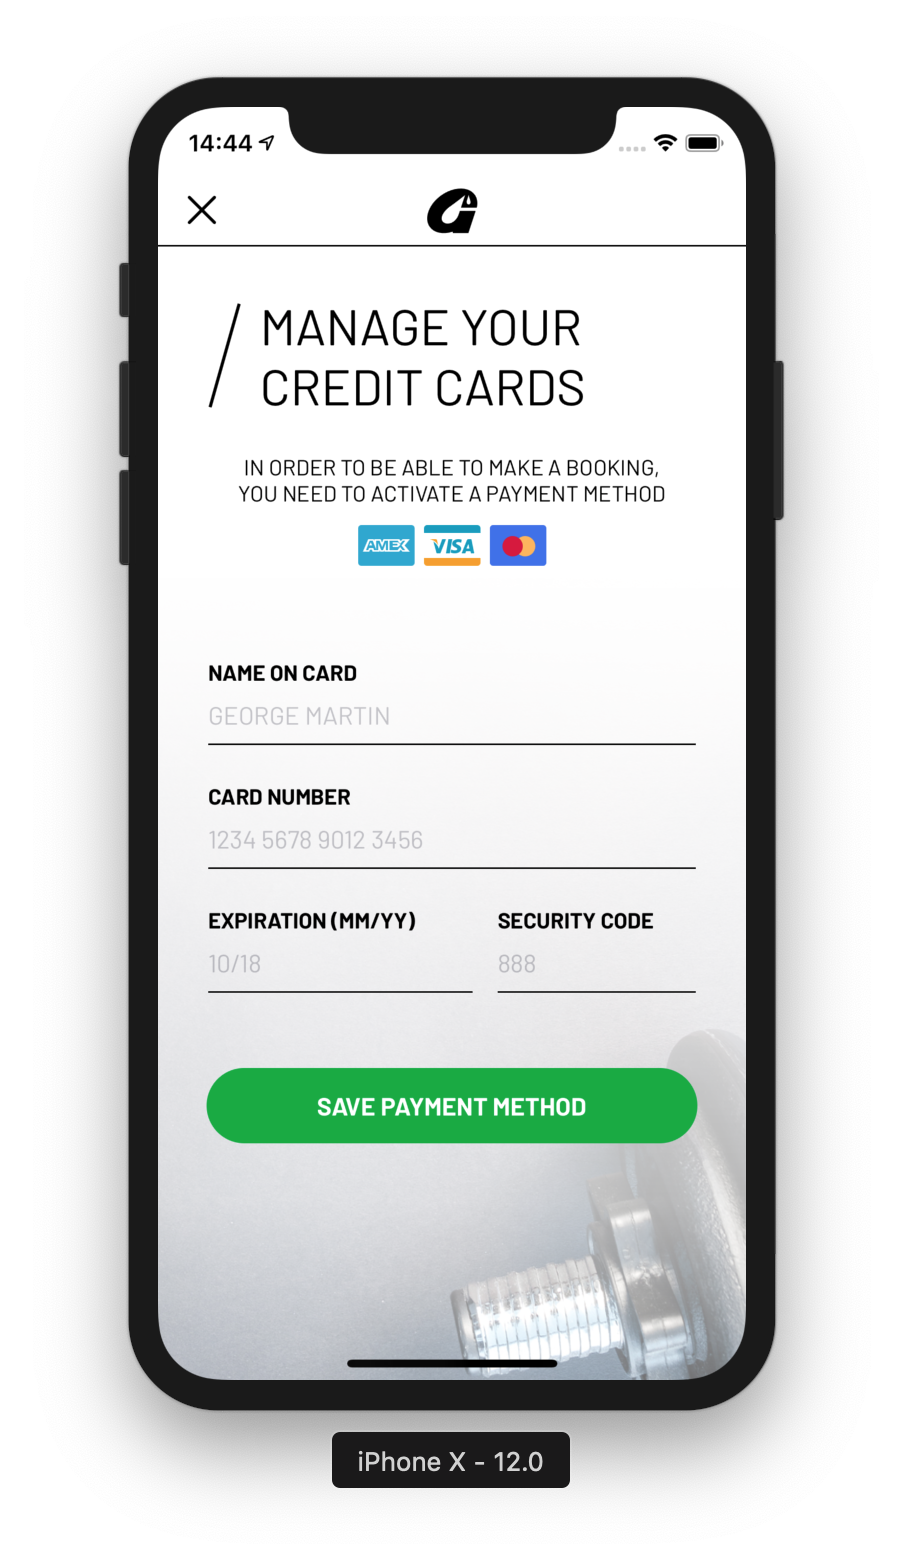
\includegraphics[width=0.14\textwidth]{pfc/figuras/add-card.png}
    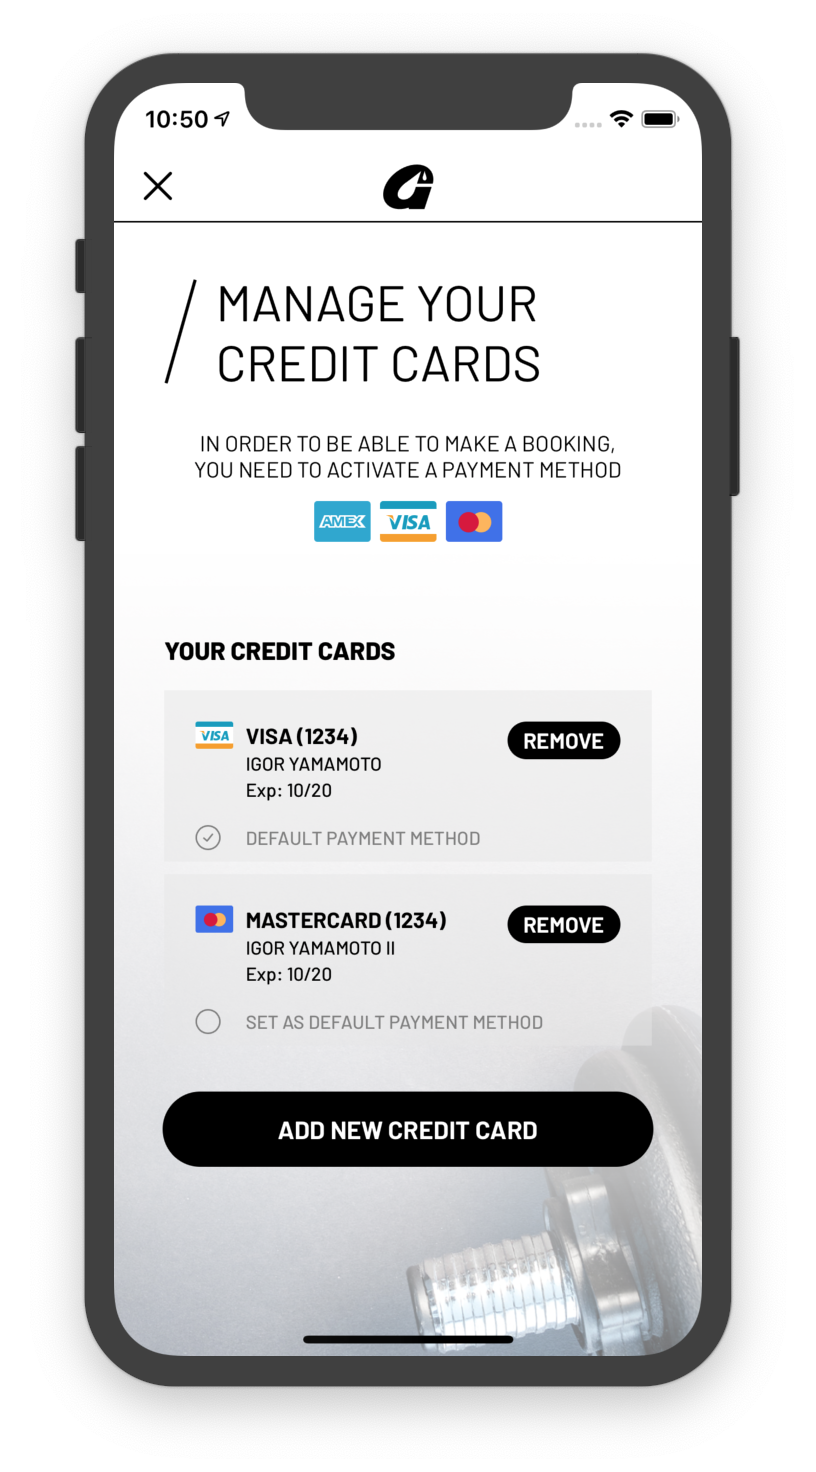
\includegraphics[width=0.14\textwidth]{pfc/figuras/manage-cards.png}
    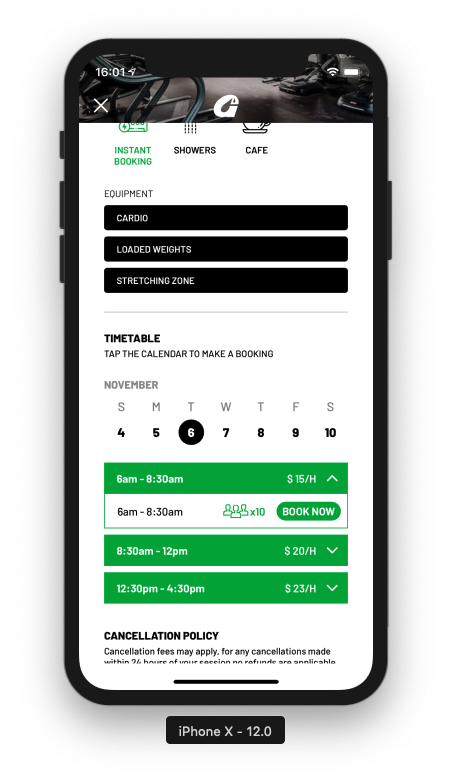
\includegraphics[width=0.14\textwidth]{pfc/figuras/tr-gym-profile-2.png}
    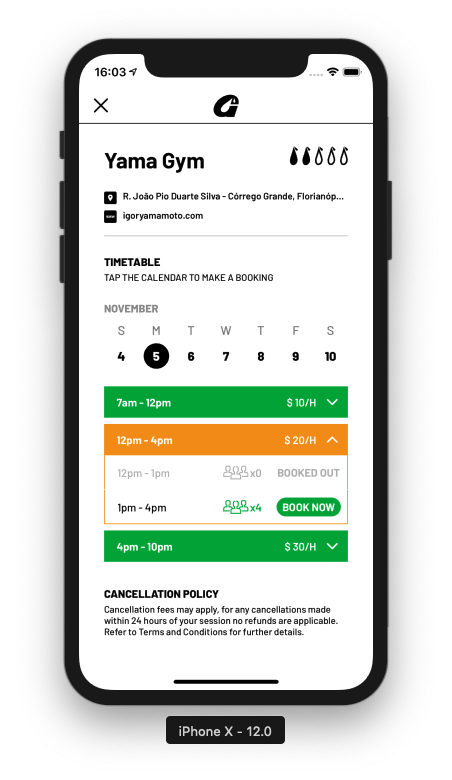
\includegraphics[width=0.14\textwidth]{pfc/figuras/tr-availability-2.png}
    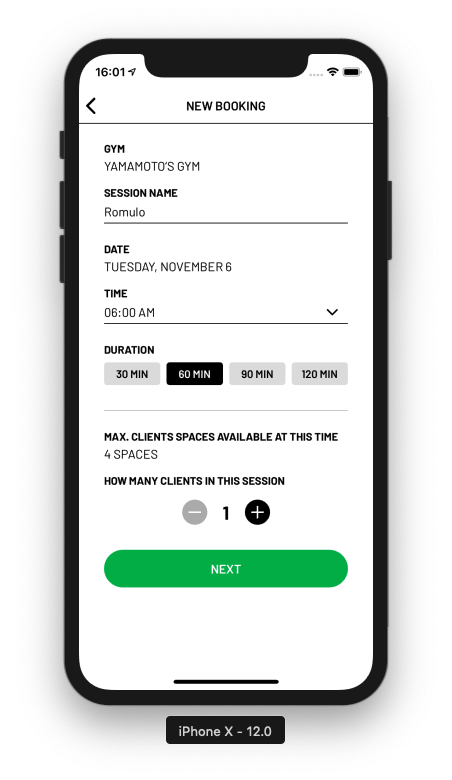
\includegraphics[width=0.14\textwidth]{pfc/figuras/tr-new-booking.png}
    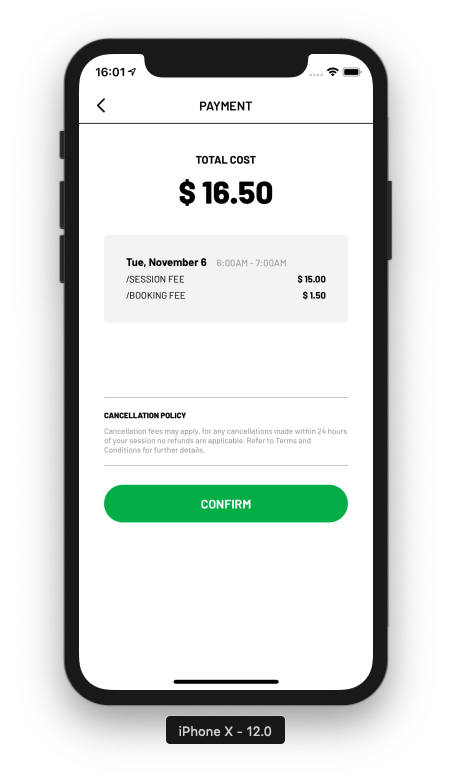
\includegraphics[width=0.14\textwidth]{pfc/figuras/tr-booking-payment.png}
    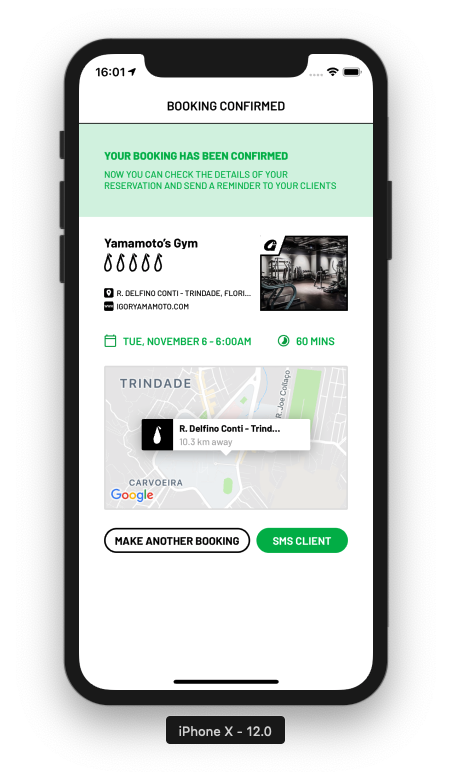
\includegraphics[width=0.14\textwidth]{pfc/figuras/tr-booking-confirmed.png}
    \caption{Todas as telas desenvolvidas para a versão piloto}
    \label{fig:all-screens}
\end{figure}

\section{Testes Automatizados}
\subsection{Comparação entre Ferramentas}
Com base em pesquisas e nas implementações dos casos de teste, foi possível traçar um comparativo entre as ferramentas a respeito dos seguintes critérios:

\begin{itemize}
    \item Setup: a configuração do EarlGrey foi de relativa facilidade, uma vez que a ferramenta utiliza o mesmo ambiente de desenvolvimento do aplicativo iOS (Xcode). Em contrapartida, o setup do Appium apresentou mais dificuldades por requerer mais etapas de configuração, incluindo instalação de outros componentes de software.
    \item Facilidade de Uso: ambas as ferramentas apresentaram baixa complexidade de uso, facilitando o desenvolvimento dos casos de teste. As API's disponíveis são de fácil entendimento e uso. 
    \item Desempenho: o desempenho das ferramentas foi avaliado com base no tempo de execução do primeiro caso de teste. Cinco rodadas de execução foram realizadas para cada uma das ferramentas, além do mesmo ser feito para a execução manual do teste. A Figura \ref{fig:box-plot-time} ilustra o resultado do experimento. O EarlGrey obteve o melhor desempenho, com tempo médio de $1$min e $47$s; em seguida encontram-se os testes manuais, com tempo médio de $1$min e $59$s; por último, o Appium obteve um tempo médio de $3$min e $2$s. O maior tempo de execução do Appium era esperado, uma vez os comandos enviados através da ferramenta para o dispositivo são intermediados por um servidor web local. Os tempos de execução foram considerados razoáveis para ambas as ferramentas frente ao cenário de uso. Contudo, para aplicações com diferentes escalas de teste, novos testes devem ser realizados.
    \item Versatilidade: o Appium mostrou-se ser mais versátil que o EarlGrey por ter suporte multiplataforma (podendo ser utilizado em sistemas iOS, Android e Web). O EarlGrey está restrito ao sistema iOS. Além disso, o Appium conta com API's em mais linguagens de programação, como Python e Javascript. O EarlGrey está restrito às linguagens de desenvolvimento iOS.
\end{itemize}

\begin{figure}[H]
    \centering
    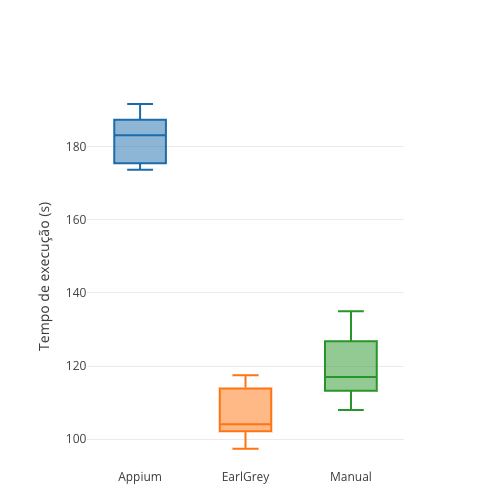
\includegraphics[width=0.8\textwidth]{pfc/figuras/box-plot-time.png}
    \caption{Comparação entre tempos de execução dos testes}
    \label{fig:box-plot-time}
\end{figure}

\subsection{Validade dos Casos de Teste}
O estudo e implementação dos casos de teste resultaram em algumas conclusões a respeito da importância da realização dos mesmos no contexto do projeto. Ambos os testes foram considerados relevantes para o teste da aplicação. Contudo a forma de realização dos mesmos pode ser melhorada para otimizar os retornos para o projeto.

O primeiro caso de teste apresentou boas perspectivas para implementações futuras em situações semelhantes. O teste teve bom desempenho em relação ao tempo de execução, superando o tempo de teste feito manualmente. O tempo de implementação do teste também foi razoável e a curto prazo pode trazer retornos ao evitar a repetição do teste manual. Além disso, o teste apresentou relevância em termos de qualidade do produto, assumindo o papel de teste de aceitação e regressão. A primeira função decorre do fato do mesmo possibilitar a validação de um fluxo de uso do aplicativo, ao interagir com diversas telas de forma a simular o comportamento real do usuário. Enquanto a última, permite que a integridade do fluxo de uso seja testada após a adição de novas funcionalidades.

O segundo teste mostrou-se importante para testar múltiplas combinações de entrada de usuário. O teste revelou falhas no design do aplicativo do ponto de vista de usabilidade, ao expor os diversos cenários de estados de erro. O mesmo também possibilitou a verificação das mensagens e estados de erro. Contudo, o teste apresentou resultados ruins em termos de desempenho de execução, chegando a ultrapassar $20$min de tempo total. Este resultado ruim indica que o teste deveria ser realizado em um nível mais baixo da camada de testes (possivelmente na camada de serviços, ao invés de ser feito a nível de interface gráfica), de forma a ficar mais próximo ao código.

\subsection{Processos da Empresa}
O estudo trouxe resultados em questão ao valor que os testes automatizados podem adicionar ao produto, ao cliente e ao time de desenvolvimento dentro da empresa. Ao introduzir a implementação de testes automatizados no projeto, o produto ganha mais uma sustentação na sua garantia de qualidade. Os testes automatizados de interface gráfica tem potencial para aumentar a satisfação do cliente, ao permitir que o mesmo visualize a integridade do produto constantemente durante sua evolução, através de gravações de vídeos e fotos de telas em diferentes tamanhos de dispositivos.

O estudo revelou a necessidade da empresa estruturar projetos de teste em níveis mais baixos, como testes unitários e na camada de serviços. Antes de investir mais tempo em testes automatizados voltados a interface gráfica, implementações podem ser feitos nas outras camadas. O segundo caso de teste apresentado neste trabalho exemplifica a necessidade, justificada pelo fato do teste ter demandado tempo que poderia ser poupado, caso o mesmo fosse implementado em camadas inferiores.

A implementação dos testes automatizados de interface gráfica mostrou-se adequada ao atual cenário de fluxo de trabalho da empresa. Este fato decorre dos testes poderem ser feitos de maneira isolada da aplicação. Pequenos ajustes podem ser realizados para permitir que o processo seja desempenhado com maior fluidez, como a adição de identificadores de acessibilidade desde o começo do projeto. Além disso, scripts podem ser criados para facilitar a chamada dos testes, abrindo possibilidade para que os testes sejam performados em mais tipos de dispositivos e paralelizados.

O estudo trouxe contribuições em relação ao que pode ser testado e a quem é atribuída a função de criar os testes de interface gráfica. Para esta camada, testes podem ser realizados para testar os principais fluxos da aplicação de maneira, garantindo a integridade contínua e a adequação às regras de negócio. Pelo fatos deste tipo de teste estar próximo ao comportamento do usuário final, todo o time pode estar envolvido na elaboração. Além disso, o fator de isolamento, em relação ao código da aplicação, permite que os testes sejam implementados e executados por mais membros técnicos da equipe.

\section{Validação do Programa de Capacitação da Empresa}
O presente trabalho esteve inserido na empresa Jungle Devs como parte do programa de capacitação do autor. O programa de capacitação \textit{Academy} não havia sido concluído por nenhuma pessoa anteriormente. Portanto, um dos resultados obtidos por este PFC para a empresa é a validação do programa.

A proposta de conclusão de um projeto de aplicação prática real, em conjunto com um time de engenharia de software, foi efetuada com sucesso. O projeto do aplicativo Gyymi para o sistema iOS se mostrou eficaz para a capacitação do autor em projetos de aplicações \textit{mobile}. Isso se deve ao fato do aplicativo contemplar a maioria das funcionalidades recorrentes em aplicativos em produção no mercado, como cadastro e autenticação de usuários, navegação customizada por múltiplas telas e integração com sistemas de software terceiros.

Além de validar a etapa final do programa \textit{Academy}, na qual o projeto do aplicativo esteve inserido, o trabalho revelou bons resultados no que diz respeito às etapas anteriores. Esta afirmação é justificada a partir da análise da contribuição prática do autor para o projeto. A partir dos dados disponíveis no repositório do código fonte da aplicação (ver Figura \ref{fig:github-stats}), é possível concluir que o autor teve contribuições significativas desde o começo do projeto. Os dados indicam a contribuição do autor em $70\%$ das linhas de código modificadas durante o projeto, totalizando $55408$ alterações. Além disso, o autor teve contribuição em $74\%$ dos incrementos de versão do código (\textit{commits}), totalizando $699$ mensagens de incremento salvas. Assim, é possível concluir que as etapas iniciais do programa de capacitação foram efetivas para a aprendizagem de conceitos práticos de projeto.
\begin{figure}[H]
    \centering
    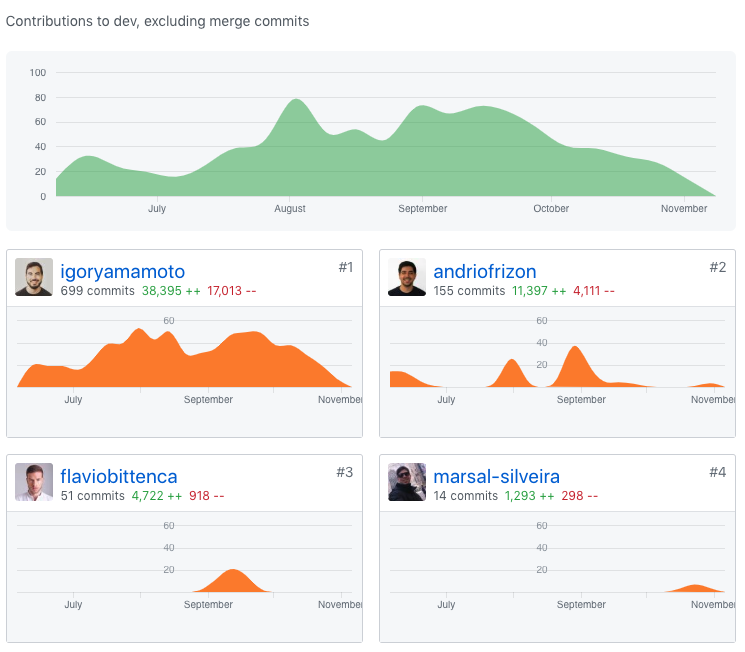
\includegraphics[width=\textwidth]{pfc/figuras/github-stats.png}
    \caption{Dados de contribuição no projeto do aplicativo iOS por membro do time}
    \label{fig:github-stats}
\end{figure}
